\documentclass{article}

\usepackage{amsmath}
\usepackage{graphicx}
\usepackage{hyperref}
\usepackage{float}
\usepackage{array}
\usepackage{listings}
\usepackage{xcolor}
\usepackage{flafter} 
\usepackage{booktabs} 
\usepackage[letterpaper,top=2cm,bottom=2cm,left=3cm,right=3cm,marginparwidth=1.75cm]{geometry}

\title{Flight Operation Report}
\author{Tech Troopers}
\date{\today}

\begin{document}

\maketitle

\begin{center}
\large{\textbf{filename.csv}}
\end{center}

\section{Flight Type}

\subsection{Class Type}
The class type for this operation has been identified as \textbf{Normal Operation Detected}.

\subsection{Confidence of Prediction}
The model used for this classification is a voting classifier. This ensemble method aggregates the predictions of the following classifiers to produce a final prediction:

\begin{itemize}
    \item \textbf{Logistic Regression}
    \item \textbf{Decision Tree Classifier}
    \item \textbf{Random Forest Classifier}
    \item \textbf{Gradient Boosting Classifier}
    \item \textbf{XGBoost Classifier}
\end{itemize}

The overall predicted probabilities for each classifier across all samples are as follows:

\begin{table}[h]
\centering
\resizebox{\textwidth}{!}{%
\begin{tabular}{|l|l|l|l|l|l|}
\hline
\textbf{Operation} & \textbf{Logistic Regression} & \textbf{Decision Tree} & \textbf{Random Forest} & \textbf{Gradient Boosting} & \textbf{XGBoost} \\ \hline
Normal Operation & 0.353389 & 0.000000 & 0.000977 & 0.052877 & 0.000220 \\ \hline
Non Normal Operation & 0.646611 & 1.000000 & 0.999023 & 0.947123 & 0.999780 \\ \hline
\end{tabular}%
}
\caption{Overall Predicted Probabilities for Each Classifier}
\label{table:overall_probabilities}
\end{table}

\begin{figure}[H]
\centering
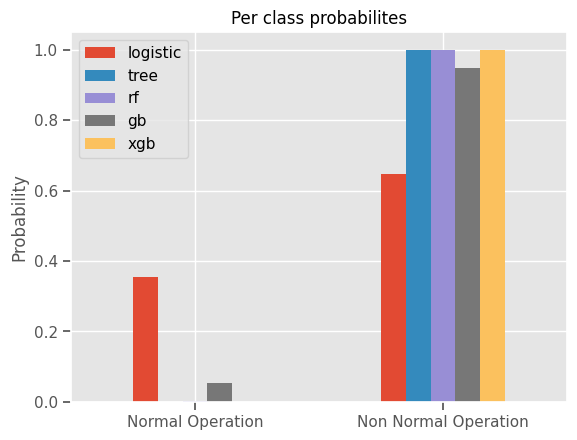
\includegraphics[width=0.57\textwidth]{img/per_class_prob.png}
\caption{Predicted Probabilities per Class}
\label{fig:class_probabilities}
\end{figure}


Each classifier provides its predicted probabilities, contributing to the final decision through majority voting, ensuring robust and accurate predictions.



\subsection{Individual Classifier Predictions}

The classification was performed using a voting classifier, which combines the predictions of several individual classifiers to improve accuracy and reliability. The ensemble consists of the following classifiers:

\begin{table}[h]
\centering
\begin{tabular}{|l|l|}
\hline
\textbf{Classifier} & \textbf{Prediction} \\ \hline
Logistic Regression & Normal Operation Detected \\ \hline
Decision Tree Classifier & Normal Operation Detected \\ \hline
Random Forest Classifier & Normal Operation Detected \\ \hline
Gradient Boosting Classifier & Normal Operation Detected \\ \hline
XGBoost Classifier & Normal Operation Detected \\ \hline
\end{tabular}
\caption{Individual Classifier Predictions}
\label{table:individual_predictions}
\end{table}

The predictions from each classifier are combined using majority voting to determine the final class type. This method ensures that the final classification result is robust and reliable, leveraging the diverse strengths of each individual model.

\section{Conclusion}
This analysis highlights the critical role of exploratory data analysis (EDA) and preprocessing in developing an effective predictive model. Through EDA, we gained valuable insights into the dataset, including the identification of key features, detection of outliers, and understanding the distribution of data. Visualizations such as histograms and scatter plots helped clarify relationships between features and their impact on the target variable.

Preprocessing steps, including handling missing values, scaling features, and encoding categorical variables, were essential for preparing the data for modeling. These steps ensured that the classifiers could effectively interpret the data without bias or noise.

Applying various classification algorithms, particularly the voting classifier, allowed us to leverage the strengths of multiple models, leading to improved prediction accuracy. Each algorithm provided unique insights, and the ensemble approach enhanced robustness against overfitting.

Overall, this process underscores the importance of a systematic approach to data analysis and model development. The lessons learned from EDA and preprocessing not only informed feature selection and engineering but also contributed significantly to the overall performance of the classification models. Future work can focus on refining these techniques and exploring advanced algorithms to further enhance predictive capabilities.


\end{document}